\documentclass{UoNMCHA}
\usepackage[authoryear]{natbib}
\usepackage{array,booktabs} % For nice tables
\usepackage{amsmath,amsfonts,amssymb} % For nice maths
\usepackage{color}
\usepackage{enumerate}
\usepackage{listings}
\usepackage{subfig}
\usepackage{hyperref}
\usepackage{pdfpages}
\usepackage{rotating}
\usepackage[parfill]{parskip}   % For replacing paragraph indenting with a newline instead
% Number equations per section
\numberwithin{equation}{section}

\hypersetup{
%    bookmarks=true,         % show bookmarks bar?
%    unicode=false,          % non-Latin characters in AcrobatÕs bookmarks
%    pdftoolbar=true,        % show AcrobatÕs toolbar?
%    pdfmenubar=true,        % show AcrobatÕs menu?
%    pdffitwindow=false,     % window fit to page when opened
%    pdfstartview={FitH},    % fits the width of the page to the window
%    pdftitle={My title},    % title
%    pdfauthor={Author},     % author
%    pdfsubject={Subject},   % subject of the document
%    pdfcreator={Creator},   % creator of the document
%    pdfproducer={Producer}, % producer of the document
%    pdfkeywords={keyword1} {key2} {key3}, % list of keywords
%    pdfnewwindow=true,      % links in new window
    colorlinks=true,       % false: boxed links; true: colored links
    linkcolor=blue,          % color of internal links
    citecolor=blue,        % color of links to bibliography
%    filecolor=magenta,      % color of file links
    urlcolor=blue           % color of external links
}

\definecolor{MATLABKeyword}{rgb}{0,0,1}
\definecolor{MATLABComment}{rgb}{0.1328125,0.54296875,0.1328125}
\definecolor{MATLABString}{rgb}{0.625,0.125,0.9375}

\lstset{language=Matlab,
    basicstyle=\small\ttfamily,
    keywordstyle=\color{MATLABKeyword},
    %identifierstyle=,
    commentstyle=\color{MATLABComment},
    stringstyle=\color{MATLABString},
    numberstyle=\tiny,
    %numbers=left,
    basewidth=0.5em}

\firstpage{1}    % Set page number for first page
\UoNMCHAreportNo{MECH4841 Part B} %Report number
\UoNMCHAyear{2013}   % Year
\shorttitle{FYP Report - Optical Flow Based Obstacle Avoidance} %For odd pages
%%%%%%%%%%%%%%%%%%%%%%%%%%%%%%%
\begin{document}

\includepdf[pages=-]{FYP_Cover_Page.pdf}
\title{Optical Flow Based Obstacle Avoidance for a Fixed Wing UAV\\ \ \\
{\small Final Year Project Report - MECH4841 Part B  \\June 2019}}
\author[UoNMCHA]{Patrick Prell}
\address[UoNMCHA]{
Student of Mechatronics Engineering,\\
The University of Newcastle, Callaghan, NSW 2308, AUSTRALIA \\
Student Number: 3204734 \\
E-mail: \href{mailto:Patrick.Prell@uon.edu.au}{\textsf{Patrick.Prell@uon.edu.au}}}
%%%%%%%%%%%%%%%%%%%%%%%%%%%%%%%
\maketitle
\onecolumn

\vspace{-5mm}
\section*{Abstract}
\vspace{-3mm}
Remember that executive summary may include the following information:
\begin{itemize}
    \item Defines the intention of the report.
    \item Places the report in context so the reader knows why it is important to read it.
    \item Why is it important?
    \item What problem is addressed?
    \item Briefly states the results
    \item Briefly presents the implications and recommendations
\end{itemize}
%%%%%%%%%%%%%%%%%%%%%%%%%%%%%%%
\vspace{-2mm}
\section*{Acknowledgements}
\vspace{-3mm}
You may like to say thank you to someone that helped you with your project.
%%%%%%%%%%%%%%%%%%%%%%%%%%%%%%%
\newpage
\tableofcontents
\newpage
%%%%%%%%%%%%%%%%%%%%%%%%%%%%%%%
\section{Introduction}

Exploring and navagating unknown environments is an essential instinct in biology and avoiding obstacles is an major component. For robotic vehicles to perform high level tasks, they must also have these instincts.

\begin{itemize}
    \item \textbf{Position}: Show there is a problem and that it is important to solve it.
    \item \textbf{Problem}: Describe the specifics of the problem you are trying to address
    \item \textbf{Proposal}: Discuss how you are going to address this problem. Use the literature to back-up your approach to the problem, or to highlight that what you are doing has not been done before
\end{itemize}

The rest of the report is organised as follows. Section~\ref{sec:Background} describes items related to the core content. Section~\ref{sec:Conclusion} concludes the report. Appendix~ shows an example of how to make a Table.

% %%%%%%%%%%%%%%%%%%%%%%%%%%%%%%%
% \newpage
\section{Background}\label{sec:Background} %Checked with grammarly
%TODO: Pretty good, get someone to read
To the average human or most mammals for that matter, visual tasks such as identifying objects and interpreting visual cues seem like a trivial task. However, implementing algorithms that mimic a mammalian visual cortex is infuriatingly difficult and largely remains an unsolved problem \citep{hartley2003multiple}. One fact often overlooked is that for all of its amazing abilities, approximately 1/3 of the human brain is dedicated to analysing information collected from our eyes. This statistic helps to put into perspective how challenging the field of computer vision can be.

The concept of computer vision has been explored since the inception of artificial intelligence in the late 1960s. Corresponding with a rise in electronic computer power, allowing manipulation of large data sets such as those collected from a camera. The following decade saw research attempting to extract information from a sequence of images using visual cues embedded in the motion of an image. This brought about research on visual navigation as a viable method for a mobile robot to navigate an environment. Using Visual Navigation on a robot to move through an unstructured environment with no prior knowledge of the map is often based on optical flow. A motion field is estimated from fusing the motion of the robot with the motion of the pixels of a video feed. Furthermore, visual navigation techniques have been inspired by biology. Observing the way that animals and insects utilise their visual systems to move about and map their environments, the processes for which this is achieved can be replicated and implemented on a robotic system \citep{altshuler2018comparison}.

The following section builds the background knowledge required to utilise visual cues as input to an obstacle avoidance system. In particular, a history of visual navigation is outlined;  the geometry of a camera and the tools for calibrating it is introduced; and the kinematics of vision optical flow and optical flow on the view sphere. Finally, this section discusses the approach taken to validate the obstacle avoidance algorithm.

% \subsection{Inverse Optimal Control} % 3 pages

\subsubsection{Biomimicry} % 1 page %Checked with grammarly
Biology so often holds a wealth of inspiration for engineers. From the material science of the microstructures in a butterfly wing to the computational fluid dynamics of a Kingfisher diving into water \citep{benyus1997biomimicry}. visual sensors are found so frequently in nature, making it very productive to look at nature and tap into the eons of knowledge distilled by evolution.

\subsubsection{Visual Navigation}
\subsubsection{Sudo Control Algorithm for Insects}
\subsubsection{}
\subsection{Optical Flow} % 2 pages %TODO: From part A Fix this up
In computer vison we are constanly running into the problem of dimentional compression. A lot of information is lost in the projection from 3 dimentions to a 2D plane, and when that projection is inverted, the lost data needs to be inferred. In the case of optical flow, the lost data comes mainly from different assumptions that are made to make the optic flow algorithm solvable. Each Optical flow algorithm has its own set of assumptions and constraints
\subsubsection{Horn \& Schunk} %TODO: From part A Fix this up
Optical flow is an ill-posed problem, meaning that there is only one independent measurement available from the image sequence and we require 2 variables to describe the flow at a point. B.K.P. Horn and B.G. Schunck developed an algorithm for computing optical flow in 1980 \citep{horn1981determining} by adding a second constraint known as the brightness constancy. The brightness constancy constraint assumes that the pixel intensities remain constant over time.

\begin{equation}
	\frac{d}{dt} I(x(t), y(t), t) = 0
\end{equation}
where $I(x(t), y(t), t)$ is the pixel intencity of the image at time $t$.

Horn and Schunck's optical flow algorithm was a huge step forward in computer vision research, although this algorithm is limited in that it typically can only estimate small motions, the method fails in the presence of large motion when the gradient of the image is not smooth enough \citep{meinhardt2013horn}.
\subsubsection{Lucas - Kanade} %TODO: From part A Fix this up
The Lucas-Kanade method is a widely used method for calculating optical flow. This method operates under the assumption that the flow is effectively constant in a small cluster of pixels, the method can then solve the optical flow equation for all the pixels in that neighbourhood using least squares regression. The Lucas-Kanade method improves on previous methods by using the spatial intensity gradient to find the disparity vector h, reducing the algorithms calculation time to $O(M^2log(N))$ for the average case.

\subsubsection{What is Observable in Optical Flow}
Pose rate estimation

\begin{itemize}
	\item Angular velocity,
	\item reflect on the work presented, 
	\item make recommendations,
	\item suggest future work or improvements.
\end{itemize}

\subsection{Camera Calibration}\label{sec:Background_cameraCal} %TODO: Pretty good, get someone to read
Computer vision begins with the camera detecting light from a scene. This light has travelled from its source, reflecting from an object, through the camera lens and is recorded on the image sensor. For these rays of light that make up an image to be useful for representing the real-world, we must understand the geometry that transforms these rays from the three-dimensional real world to a two-dimensional image plane i.e. world coordinates to image coordinates.

The camera calibration process describes the camera with two sets of parameters, namely the intrinsic parameters, and the extrinsic parameters. The intrinsic parameters describe the geometric relationship between the camera model and its projection. And the extrinsic parameters describe the location and orientation or pose, of the camera with respect to the world frame.

This project uses a GoPro Hero 7 to test and verify the calibration routine. This section will cover camera models and outline why a planar model is used for the GoPro. It covers the mathematical tools used to capture the different effects that make our camera imperfect for representing the real world, and how we can correct for these deviations.
\subsubsection{Camera Models}
The most elementary way of representing a camera is with the pinhole model. Light enters the aperture (pinhole) after reflecting from objects in a scene. For an ideal pinhole camera, only one ray enters the aperture from any point in the scene. The light is then projected onto a surface behind the aperture resulting in an image of the scene that is scaled proportionally to the focal length $f$.

\begin{figure}[ht]
    \begin{center}
        \includegraphics[width=.8\linewidth]{Figures/Pinhole_model}
        \caption{Elementary pinhole model of a camera: In practice, the appeture must be big enough to let light in, allowing a narrow ray of light from each point in the scene blurring the image. Therefore there is a tradeoff between brightness and sharpness.}
        \label{fig:PinholeModel}
    \end{center}
\end{figure}

Figure~\ref{fig:PinholeModel} shows an ideal pinhole camera model and its parameters, where $f$ is the focal length, $Z$ is the distance along the optical axis to an object, $x$ is the size of the projected object and $X$ is the size of the object. For this model, \eqref{eq:pinholeEQ} is the relationship between the projected image and the object
\begin{equation}\label{eq:pinholeEQ}
	\frac{-x}{f} = \frac{X}{Z}
\end{equation}
Due to how light enters the camera, the image projection from a pinhole model is projected upside down. This issue is fixed in a planar camera model. The planar model is similar to a pinhole model, however rather than passing through an aperture, light travels from each point in the scene, intersects the image plane and converges to a single point known as the \textit{Centre of projection}. Figure~\ref{fig:PlainarModel} shows an ideal planar camera model. It better represents the geometry of a camera with a lens, albeit a camera with an impossibly perfect lens.

\begin{figure}[ht]
	\begin{minipage}[c]{0.3\linewidth}
		\centering
		\begin{tabular}{l l}
			$C$ &: Centre of projection\\
			$\{c\}$ &: Camera co-ordinates\\
			$P$ &: Point in world space\\
			$P'$ &: Point on image plane\\
			$\vec{u}, \vec{v}$ &: Image co-ordinates\\
			$f$ &: Focal length\\
			$I$ &: Image plane
		\end{tabular}
	\end{minipage}
	\begin{minipage}[c]{0.65\linewidth}
		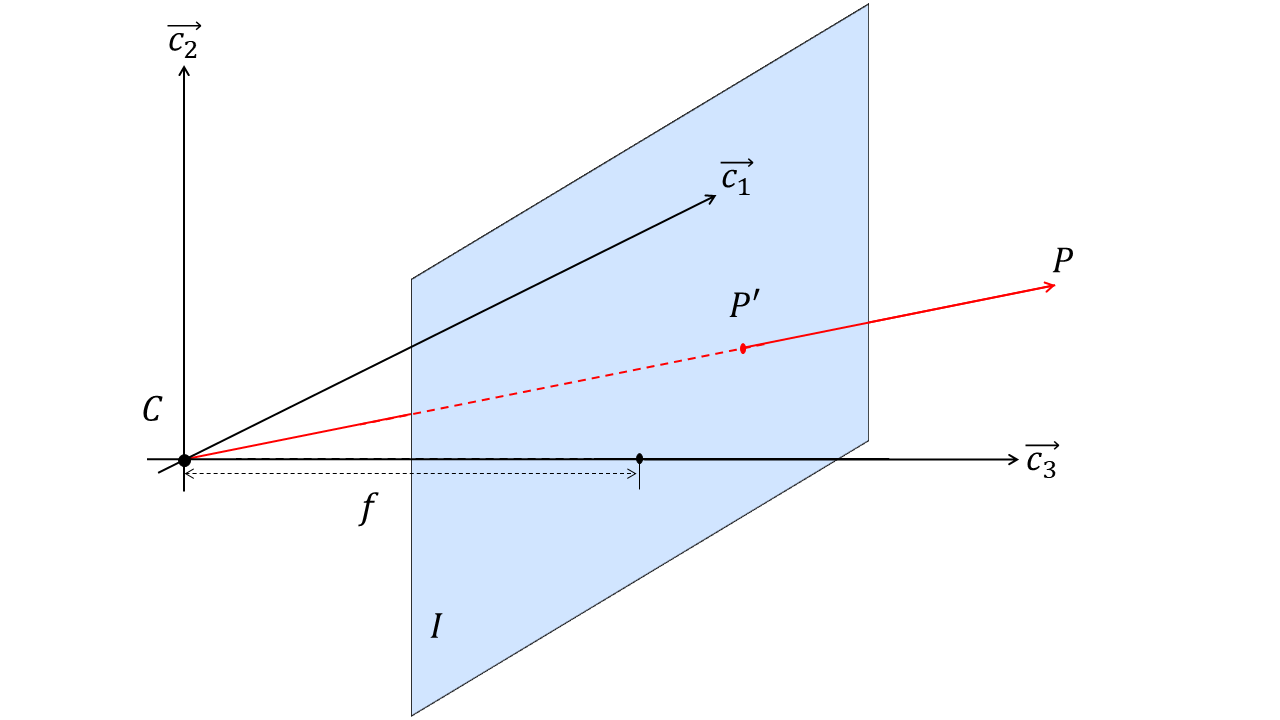
\includegraphics[width=1\linewidth]{Figures/Planar_Model}	
	\end{minipage}
\caption{Ideal camera model. A point $P$ in camera co-ordinates \{$\vec{c_{1}}, \vec{c_{2}}, \vec{c_{3}}$\} is projected and displayed as a point $p$ in image co-ordinates \{$\vec{u}, \vec{v}$\}}
\label{fig:PlainarModel}
\end{figure}
The idea behind modelling and calibrating a camera is to identify and cancel out imperfections caused by slight defects in the manufacturing process. Firstly, the image sensor is often mounted askew from the optical centre of the lens. Therefore, we introduce $\alpha_{x}$ and $\alpha_{x}$ to model a displacement from the optical centre. Furthermore, each pixel is not necessarily square causing a small discrepancy between the focal length in the $\vec{u}$ and $\vec{v}$ directions, captured in the $f_{u}$ and $f_{v}$ parameters. The following equations~\ref{eq:ProjectionEquations} project a point $P_{c_{1}, c_{2}, c_{3}}$ to image sensor co-ordinates $u, v$:
\begin{equation*}\label{eq:ProjectionEquations}
	\begin{split}
		u = &f_{u} \times \frac{\vec{c_{1}}}{\vec{c_{3}}} + \alpha_{u}\\
		v = &f_{v} \times \frac{\vec{c_{2}}}{\vec{c_{3}}} + \alpha_{v}
	\end{split}
\end{equation*}
\subsubsection{Projective Geometry}
Projective geometry is a way to describe the relationship that transforms a point from world coordinates ($n_1, n_2, n_3$) into image coordinates {$u, v$}. When applying such transformations, it is convenient to add an extra dimension to each vector in the transform. for instance, a point that lies in a $n$ dimensional space is represented in homogeneous coordinate as a $n+1$ dimensional vector. this coordinate system is known as \textit{homogenius coordinates}. for example, a point lying on a plane at $(x, y)$ is represented by the homogenous coordinates $(x, y, z)$. It is important to note that in homogeneous coordinates, any two vectors that share a common factor represents the same point in Euclidean geometry. This has the effect that a point in Euclidean geometry can be represented by an infinite number of homogeneous vectors. for instance $\alpha * (q_{1}, q_{2}, q_{3}) = (q_{1}, q_{2}, q_{3})$. The original primitive point is recovered by dividing through by $q_{3}$.


\subsubsection{Lens Distortion}
 
\subsection{Approach}
\subsubsection{Unity Simulation}
\subsection{Divergence}
\subsubsection{Assumptions}
As discussed in 

Static environment
using GoPro
Simple aircraft kinematic model
\subsubsection{Simulations}
Kinematic data collected
Used ray cast to gather depth information
\subsubsection{Real World Data}
The project is primaritly simmulation based. However, the camera calibration routine (explored in following sections was tested and evaluated on real world images collected from a GoPro Hero 7. Were this project to be implemented on a real world fixed wing UAV, the kinematic data would need to be obtained through sensors on the UAV. Additionally, the control algorithm
GoPro Hero
%%%%%%%%%%%%%%%%%%%%%%%%%%%%%%%
\newpage
\section{Optical Flow - Simulation}
\subsection{Measurement Model}
\subsection{Farnback Algorithm - OpenCV}

%%%%%%%%%%%%%%%%%%%%%%%%%%%%%%%
\newpage
\section{Camera Calibration}
As discussed in section~\ref{sec:Background_cameraCal} it is impericive to understand and account for the construction adn imperfections in a camera, if the measurments takne need to be relevent outside the camera basis $C$. This section outlines the procedure used in this project to correct a gopro hero 7 using a planar camera model and a 6th order equation to correct for distortion parameters.
\subsection{Calibration Boards}
Theoretically, to calibrate a camera any object could be used as a calibration object, so log as it is appropriately characterised. However it is much more practical to use a well defined and easily defined object. For this reason, a flat rigid checker pattern was chosen. The geometry of the calibration pattern can be seen in \ref{fig:cornerLocations}:

\begin{figure}[ht]
    \begin{center}
        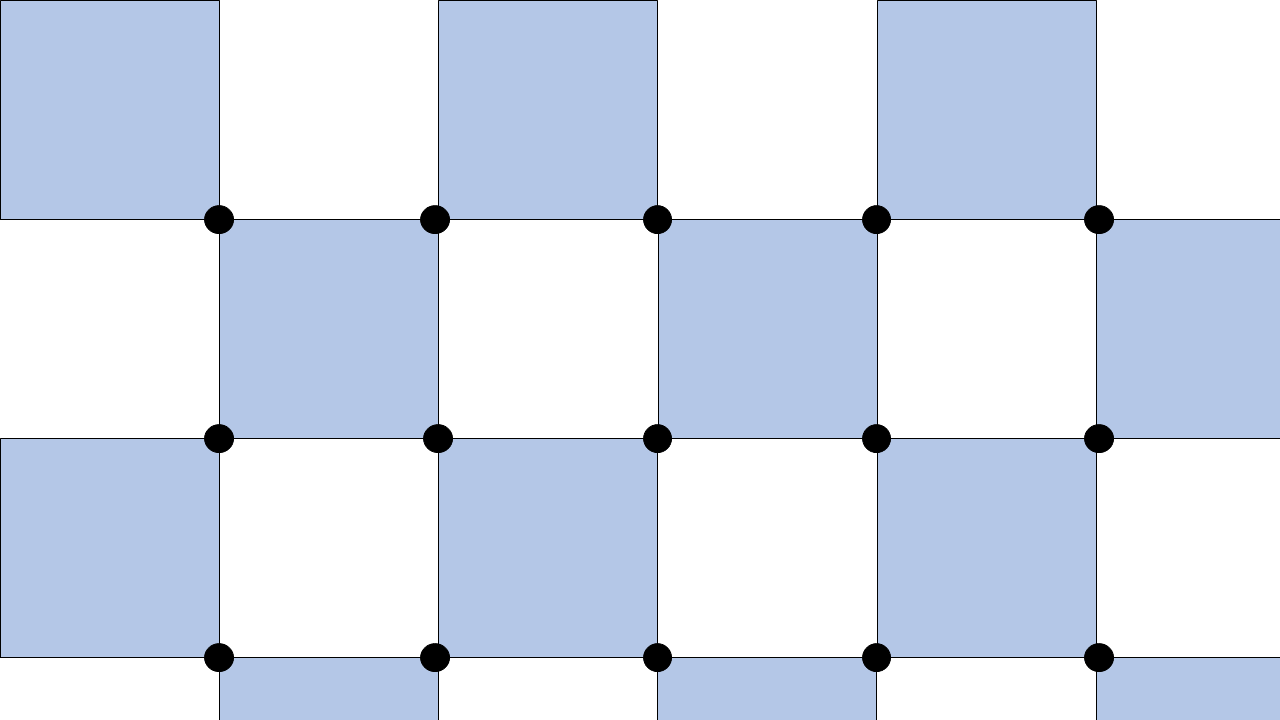
\includegraphics[width=.6\linewidth]{Figures/CalibCornerLocations}
        \caption{Write something here}
        \label{fig:cornerLocations}
    \end{center}
\end{figure}


\subsection{Calibration Tool}
To calibrate the GoPro Hero 7 for in this project, A camera calibration tool was written in C\# using WPF as a graphical user interface(see Appendix \ref{app:calibrationTool})). 

%%%%%%%%%%%%%%%%%%%%%%%%%%%%%%%
\newpage
\section{Vector Field Divergence for Object Avoidance}

%%%%%%%%%%%%%%%%%%%%%%%%%%%%%%%
\newpage
\section{Flow Magnatude for Object Avoidance}

%%%%%%%%%%%%%%%%%%%%%%%%%%%%%%%
\newpage
\section{Discussion}

%%%%%%%%%%%%%%%%%%%%%%%%%%%%%%%
\newpage
\section{Conclusion}\label{sec:Conclusion}

%%%%%%%%%%%%%%%%%%%%%%%%%%%%%%%
\newpage
\section{Recomendations}

%%%%%%%%%%%%%%%%%%%%%%%%%%%%%%%
\newpage
\bibliographystyle{harvard}
\bibliography{main} % This is the .bib file where the bibliography database is stored

%%%%%%%%%%%%%%%%%%%%%%%%%%%%%%%
\appendix
\newpage
\section{Journal}\label{app:Journal}
\newpage
\section{Calibration Tool}\label{app:calibrationTool}
\begin{figure}[ht]
    \begin{center}
        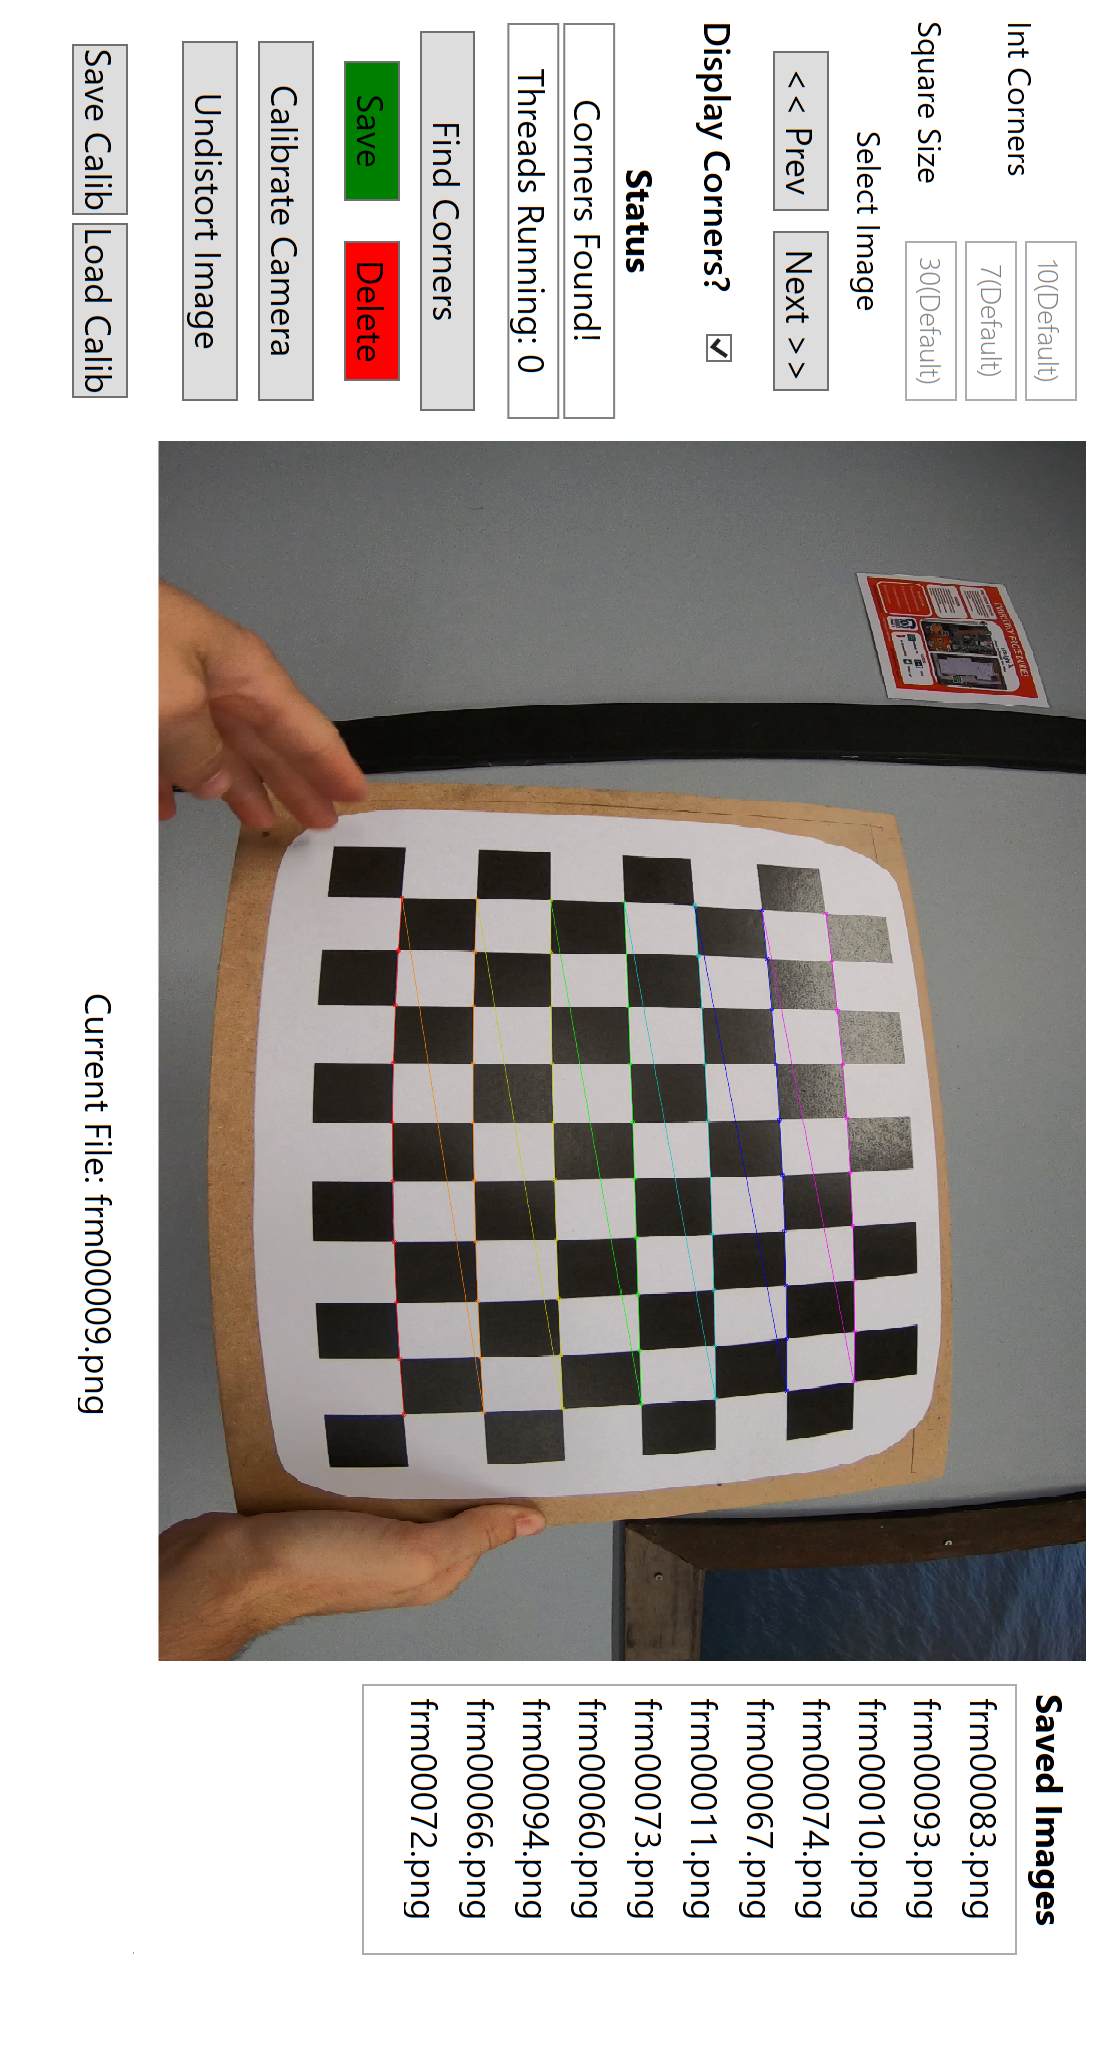
\includegraphics[width=.6\linewidth]{Figures/Calibration_Tool}
        \caption{Write something here}
        \label{fig:PinholeModel}
    \end{center}
\end{figure}

\end{document}